\section{Experiments}
\label{sec:experiments}

We (i) reproduce DiffusionOPD on SD3.5-Medium and confirm it matches the original
(\S\ref{sec:exp-repro}), then (ii) compare CA-OPD against uniform DiffusionOPD at
matched training steps, showing a convergence-efficiency benefit but comparable
final per-axis quality (\S\ref{sec:exp-caopd}). The four-idea ablation is in
\S\ref{sec:ablation}.

\subsection{Setup}
\label{sec:exp-setup}

We follow DiffusionOPD~\cite{li2026diffusionopd} and DiffusionNFT~\cite{zheng2025diffusionnft}.
The base model is SD3.5-Medium~\cite{esser2024scaling} at $512{\times}512$; the
student is a LoRA adapter ($r{=}32$, $\alpha{=}64$) trained by on-policy
distillation and evaluated with a 40-step first-order ODE sampler. We use three
task teachers---GenEval, OCR, and Aesthetics---trained once per task, and distill
them into one student. Rewards are the base method's suite: rule-based GenEval~\cite{ghosh2023geneval}
and OCR, and model-based PickScore~\cite{kirstain2023pick}, ClipScore~\cite{hessel2021clipscore},
HPSv2.1~\cite{wu2023human}, and Aesthetics~\cite{schuhmann2022aesthetics}, with
GenEval/OCR on their FlowGRPO splits and model-based rewards on
DrawBench~\cite{saharia2022photorealistic}. Unless noted, evaluation uses
$n{=}256$ prompts at student guidance scale $4.5$. We report \emph{per-axis}
metrics only. A single min-max--normalized average (as in the base method's
\textbf{Average} column) is normalization-dependent---its value shifts with the
choice of reference floor/ceiling, so it is not comparable across papers---and is
additionally circular with a min-max method (\S\ref{sec:th-conv}); we therefore
compare per axis, on which our reproduction matches DiffusionOPD
(Table~\ref{tab:repro}).

\subsection{Faithful reproduction of DiffusionOPD}
\label{sec:exp-repro}

Table~\ref{tab:repro} reports our reproduced base model, single-task teachers, and
distilled student (our uniform \texttt{mopd} checkpoint at step 721) alongside the
published numbers. All rows agree within evaluation noise: the base SD3.5-M
(with/without CFG), each teacher's in-domain peak (GenEval $0.97$, OCR $0.94$, Aes
$6.22$/HPS $0.347$), and the distilled student across all six axes. Our student
additionally cross-checks against the released official student ($\approx$
identical), giving a triple-validated reproduction.

\begin{table}[t]
\centering
\caption{\textbf{Faithful reproduction of DiffusionOPD} on SD3.5-Medium. ``Paper''
values are from~\cite{li2026diffusionopd} (Table~1); ``Ours'' are our reproduction
($n{=}256/512$). ``\texttt{mopd}@721'' is our reproduced uniform DiffusionOPD
student; it matches the paper and the released official student. Dashes: metric
not separately re-measured for that row.}
\label{tab:repro}
\small
\setlength{\tabcolsep}{4pt}
\begin{tabular}{llcccccc}
\toprule
\textbf{Model} & \textbf{Src} & \textbf{GenEval} & \textbf{OCR} & \textbf{Pick} & \textbf{Clip} & \textbf{HPS} & \textbf{Aes} \\
\midrule
\multirow{2}{*}{SD3.5-M (w/o CFG)} & Paper & 0.24 & 0.12 & 20.51 & 0.237 & 0.204 & 5.13 \\
                                   & Ours  & 0.32 & 0.11 & 20.6  & 0.238 & 0.201 & 5.18 \\
\multirow{2}{*}{\quad + CFG}       & Paper & 0.63 & 0.59 & 22.34 & 0.285 & 0.279 & 5.36 \\
                                   & Ours  & 0.59 & 0.56 & 22.4  & 0.286 & 0.283 & 5.42 \\
\midrule
\multirow{2}{*}{GenEval Teacher}   & Paper & 0.96 & 0.40 & 22.04 & 0.274 & 0.248 & 5.24 \\
                                   & Ours  & 0.97 & 0.42 & 22.0  & --    & --    & --   \\
\multirow{2}{*}{OCR Teacher}       & Paper & 0.65 & 0.93 & 22.27 & 0.290 & 0.272 & 5.26 \\
                                   & Ours  & --   & 0.94 & 22.3  & --    & --    & --   \\
\multirow{2}{*}{Aes Teacher}       & Paper & 0.49 & 0.59 & 24.02 & 0.295 & 0.346 & 6.22 \\
                                   & Ours  & --   & --   & 24.0  & 0.296 & 0.347 & 6.22 \\
\midrule
\multirow{2}{*}{\textbf{DiffusionOPD} (Ours=\texttt{mopd}@721)} & Paper & 0.96 & 0.94 & 23.99 & 0.297 & 0.342 & 6.15 \\
                                   & Ours  & 0.958 & 0.939 & 23.98 & 0.298 & 0.342 & 6.172 \\
\bottomrule
\end{tabular}
\end{table}

\subsection{CA-OPD vs.\ uniform DiffusionOPD}
\label{sec:exp-caopd}

We compare CA-OPD ($\tau{=}0.5$, $\beta{=}0.9$) against uniform \texttt{mopd} at
\emph{matched} training steps. The two arms share teachers, data, rollout, and
optimizer, differing only in the per-teacher weighting, so any difference is
attributable to the reweighting. Table~\ref{tab:caopd} reports both an early
checkpoint (@541) and convergence (@721/@781); Figure~\ref{fig:conv} plots the
training-reward proxy and the evaluation trajectory.

\paragraph{Convergence efficiency (the win).}
CA-OPD's target is the lagging axis. At the \emph{early} step 541, CA-OPD already
reaches an aesthetic score of $6.172$---the value uniform \texttt{mopd} only
attains at its own best checkpoint 721---i.e.\ roughly $180$ steps earlier
(Table~\ref{tab:caopd}, Fig.~\ref{fig:conv}). The same early checkpoint also leads
on GenEval ($0.955$ vs.\ \texttt{mopd} $0.947$), with a small OCR trade
($0.927$ vs.\ $0.939$). This is the concrete, honest benefit: faster convergence
on the hardest-to-match reward axis, exactly the min-max reallocation predicted in
\S\ref{sec:theory} (lagging axis up, saturated OCR axis slightly down).

\paragraph{Final quality (no win, stated plainly).}
By convergence the picture reverses per axis: uniform \texttt{mopd} keeps
improving while CA-OPD plateaus early. At step 721/781, CA-OPD is within
single-seed $n{=}256$ noise of \texttt{mopd} on every axis and \emph{exceeds it on
none}---GenEval, Pick, Clip, and HPS are tied, while OCR ($0.928$ vs.\ $0.939$)
and Aesthetics ($6.157$/$6.145$ vs.\ $6.172$) are marginally lower. CA-OPD's
aesthetic peak in fact drifts down after its early maximum
($6.172\!\to\!6.157\!\to\!6.145$) as min-max continuously re-chases the momentary
worst axis. \textbf{CA-OPD does not improve final per-axis quality on this
benchmark.} The temperature $\tau$ is thus best read as a speed-vs-final-quality
knob: lower $\tau$ accelerates the lagging axis but plateaus sooner;
$\tau\to\infty$ recovers \texttt{mopd}'s slower-but-higher trajectory.

\begin{table}[t]
\centering
\caption{\textbf{CA-OPD vs.\ uniform DiffusionOPD at matched steps} ($n{=}256$,
gs $4.5$; per-axis metrics only). CA-OPD leads early (@541, driven by the
aesthetics axis, \textbf{bold}) but does not exceed \texttt{mopd} on any axis at
convergence (@721/@781); per-axis differences at convergence are within
single-seed noise.}
\label{tab:caopd}
\small
\setlength{\tabcolsep}{5pt}
\begin{tabular}{lcccccc}
\toprule
\textbf{Model} & \textbf{GenEval} & \textbf{OCR} & \textbf{Pick} & \textbf{Clip} & \textbf{HPS} & \textbf{Aes} \\
\midrule
\multicolumn{7}{l}{\emph{Early (step 541)}}\\
\texttt{mopd}@541   & 0.947 & 0.939 & 23.92 & 0.297 & 0.340 & 6.120 \\
\textbf{CA-OPD}@541 & 0.955 & 0.927 & 23.95 & 0.297 & 0.341 & \textbf{6.172} \\
\midrule
\multicolumn{7}{l}{\emph{Converged (step 721 / 781)}}\\
\texttt{mopd}@721   & 0.958 & 0.939 & 23.98 & 0.298 & 0.342 & 6.172 \\
\textbf{CA-OPD}@721 & 0.959 & 0.928 & 23.96 & 0.296 & 0.342 & 6.157 \\
\textbf{CA-OPD}@781 & 0.953 & 0.947 & 24.00 & 0.296 & 0.343 & 6.145 \\
\bottomrule
\end{tabular}
\end{table}

\begin{figure}[t]
  \centering
  % TODO(figures agent): convergence_reward.pdf, convergence_evalscore.pdf pending.
  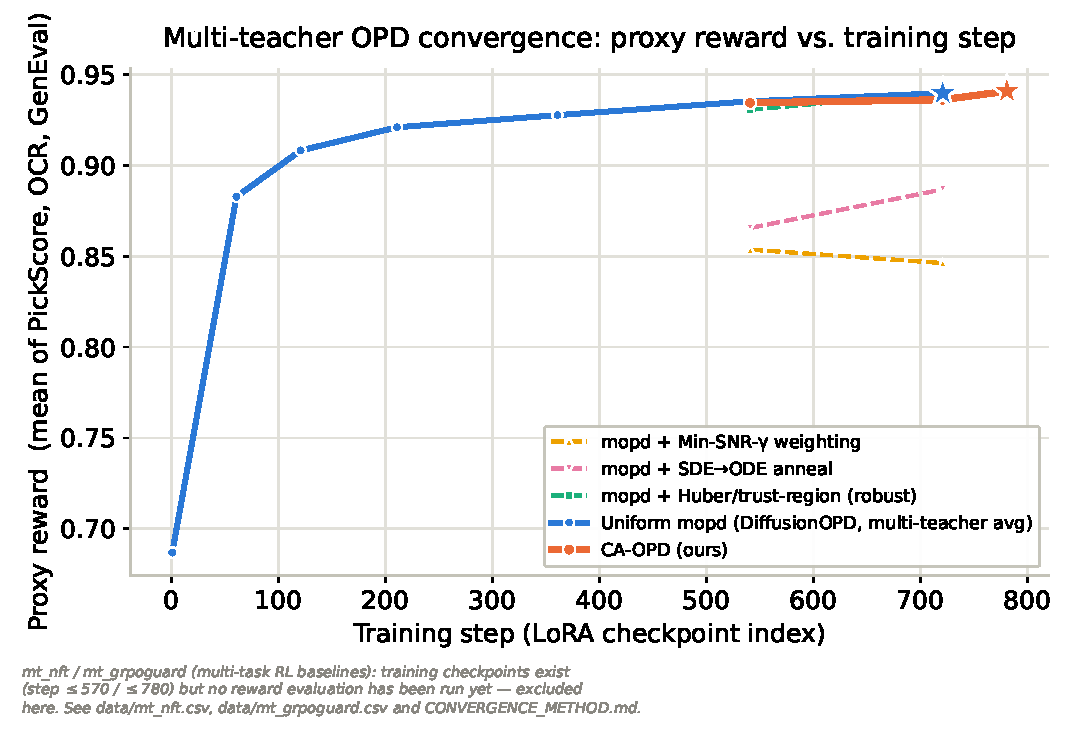
\includegraphics[width=0.48\linewidth]{figures/convergence_reward.pdf}\hfill
  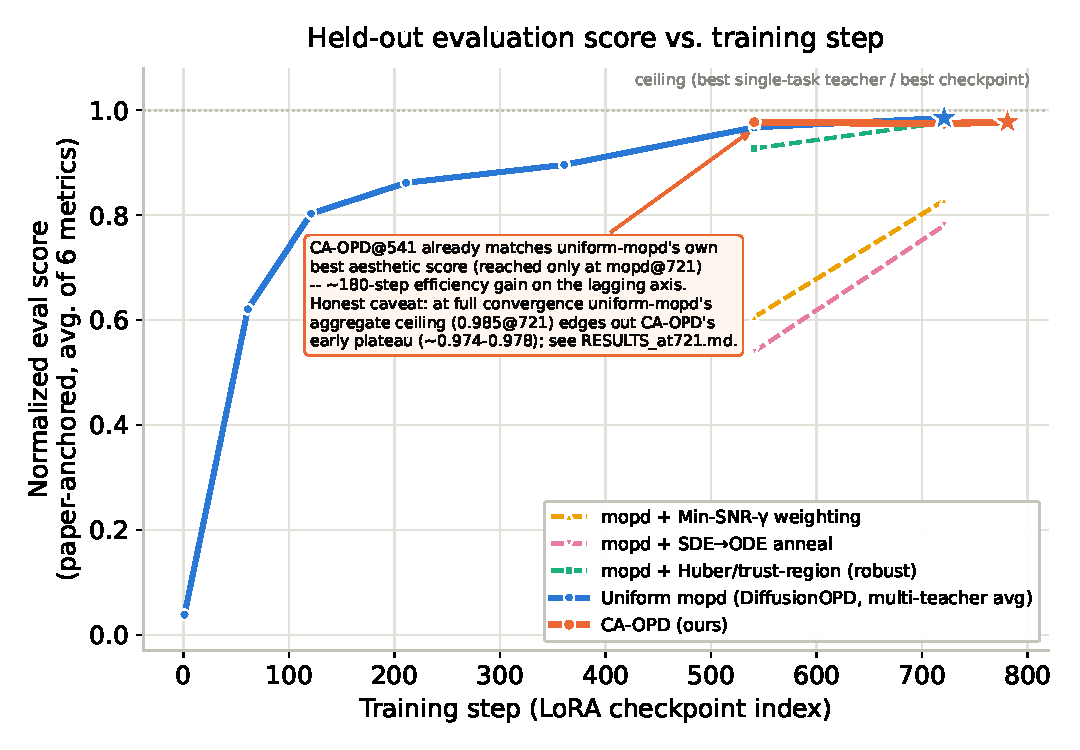
\includegraphics[width=0.48\linewidth]{figures/convergence_evalscore.pdf}
  \caption{\textbf{Convergence of CA-OPD vs.\ uniform DiffusionOPD.} Left:
  training-reward proxy vs.\ steps. Right: a normalization-dependent aggregate
  evaluation score vs.\ steps, shown for \emph{trend only} (we compare per axis in
  the tables). CA-OPD (min-max reweighting) rises faster early and reaches the
  lagging aesthetic axis $\sim$180 steps sooner, but plateaus while uniform
  \texttt{mopd} keeps improving to a slightly higher final per-axis quality.}
  \label{fig:conv}
\end{figure}

\subsection{Comparison with multi-task RL baselines}
\label{sec:exp-baselines}
Table~\ref{tab:baselines} places the OPD-distilled students against \emph{direct} multi-task
reinforcement learning---the DiffusionOPD baselines Multi-Task NFT and Multi-Task GRPO-Guard, each
jointly trained on the same three reward tasks by alternating datasets. Consistent with the original
paper, the OPD-distilled students dominate the RL baselines on \emph{every} axis: uniform-mopd and
CA-OPD are higher than both Multi-Task GRPO-Guard (@960) and Multi-Task NFT on GenEval, OCR, PickScore,
ClipScore, HPS, and Aesthetics alike (e.g.\ Aes $6.15$--$6.17$ vs.\ $5.64$/$4.91$; PickScore $24.0$ vs.\
$22.9$/$21.3$). Notably, our Multi-Task NFT run \emph{collapses} after step $\sim$570 (every metric
falls to near-zero by step 690), consistent with DiffusionNFT's documented susceptibility to
reward-hacking~\cite{zheng2025diffusionnft}; we therefore report its best (pre-collapse) checkpoint,
and this instability is itself a motivation for OPD-style distillation over direct multi-task RL.
Multi-Task GRPO-Guard trains stably and is still slowly improving (a conservative lower bound). For
reference, the original paper's own converged \emph{Average} scores---on \emph{its} normalization, which
we do not reproduce for our runs---are $0.763$ (GRPO-Guard) and $0.715$ (NFT) vs.\ DiffusionOPD $0.929$,
telling the same qualitative story. The ordering \textbf{OPD distillation $\gg$ direct multi-task RL} is
unambiguous per axis, which is the premise CA-OPD builds on.

\begin{table}[t]
\centering
\caption{\textbf{OPD distillation vs.\ direct multi-task RL} ($n{=}256$, gs $4.5$; per-axis metrics
only). Multi-task RL baselines are at their latest available checkpoints and still converging (lower
bounds). The OPD-distilled students exceed both RL baselines on every axis.}
\label{tab:baselines}
\small
\setlength{\tabcolsep}{5pt}
\begin{tabular}{lcccccc}
\toprule
\textbf{Method} & \textbf{GenEval} & \textbf{OCR} & \textbf{Pick} & \textbf{Clip} & \textbf{HPS} & \textbf{Aes} \\
\midrule
Multi-Task NFT (@570)         & 0.639 & 0.854 & 21.34 & 0.280 & 0.240 & 4.907 \\
Multi-Task GRPO-Guard (@960)  & 0.757 & 0.849 & 22.94 & 0.291 & 0.308 & 5.637 \\
\midrule
uniform DiffusionOPD (Ours, @721) & \textbf{0.958} & 0.939 & 23.98 & \textbf{0.298} & 0.342 & \textbf{6.172} \\
\textbf{CA-OPD} (@781)            & 0.953 & \textbf{0.947} & \textbf{24.00} & 0.296 & \textbf{0.343} & 6.145 \\
\bottomrule
\end{tabular}
\end{table}

\paragraph{Qualitative comparison.}
Figure~\ref{fig:qual} shows cherry-picked samples for shared prompts. CA-OPD's
early checkpoints render more polished, aesthetically richer images than
same-step \texttt{mopd}, consistent with the accelerated aesthetics axis;
differences at convergence are subtle, matching the near-tied per-axis numbers.

\begin{figure}[t]
  \centering
  % TODO(figures agent): qualitative.pdf pending.
  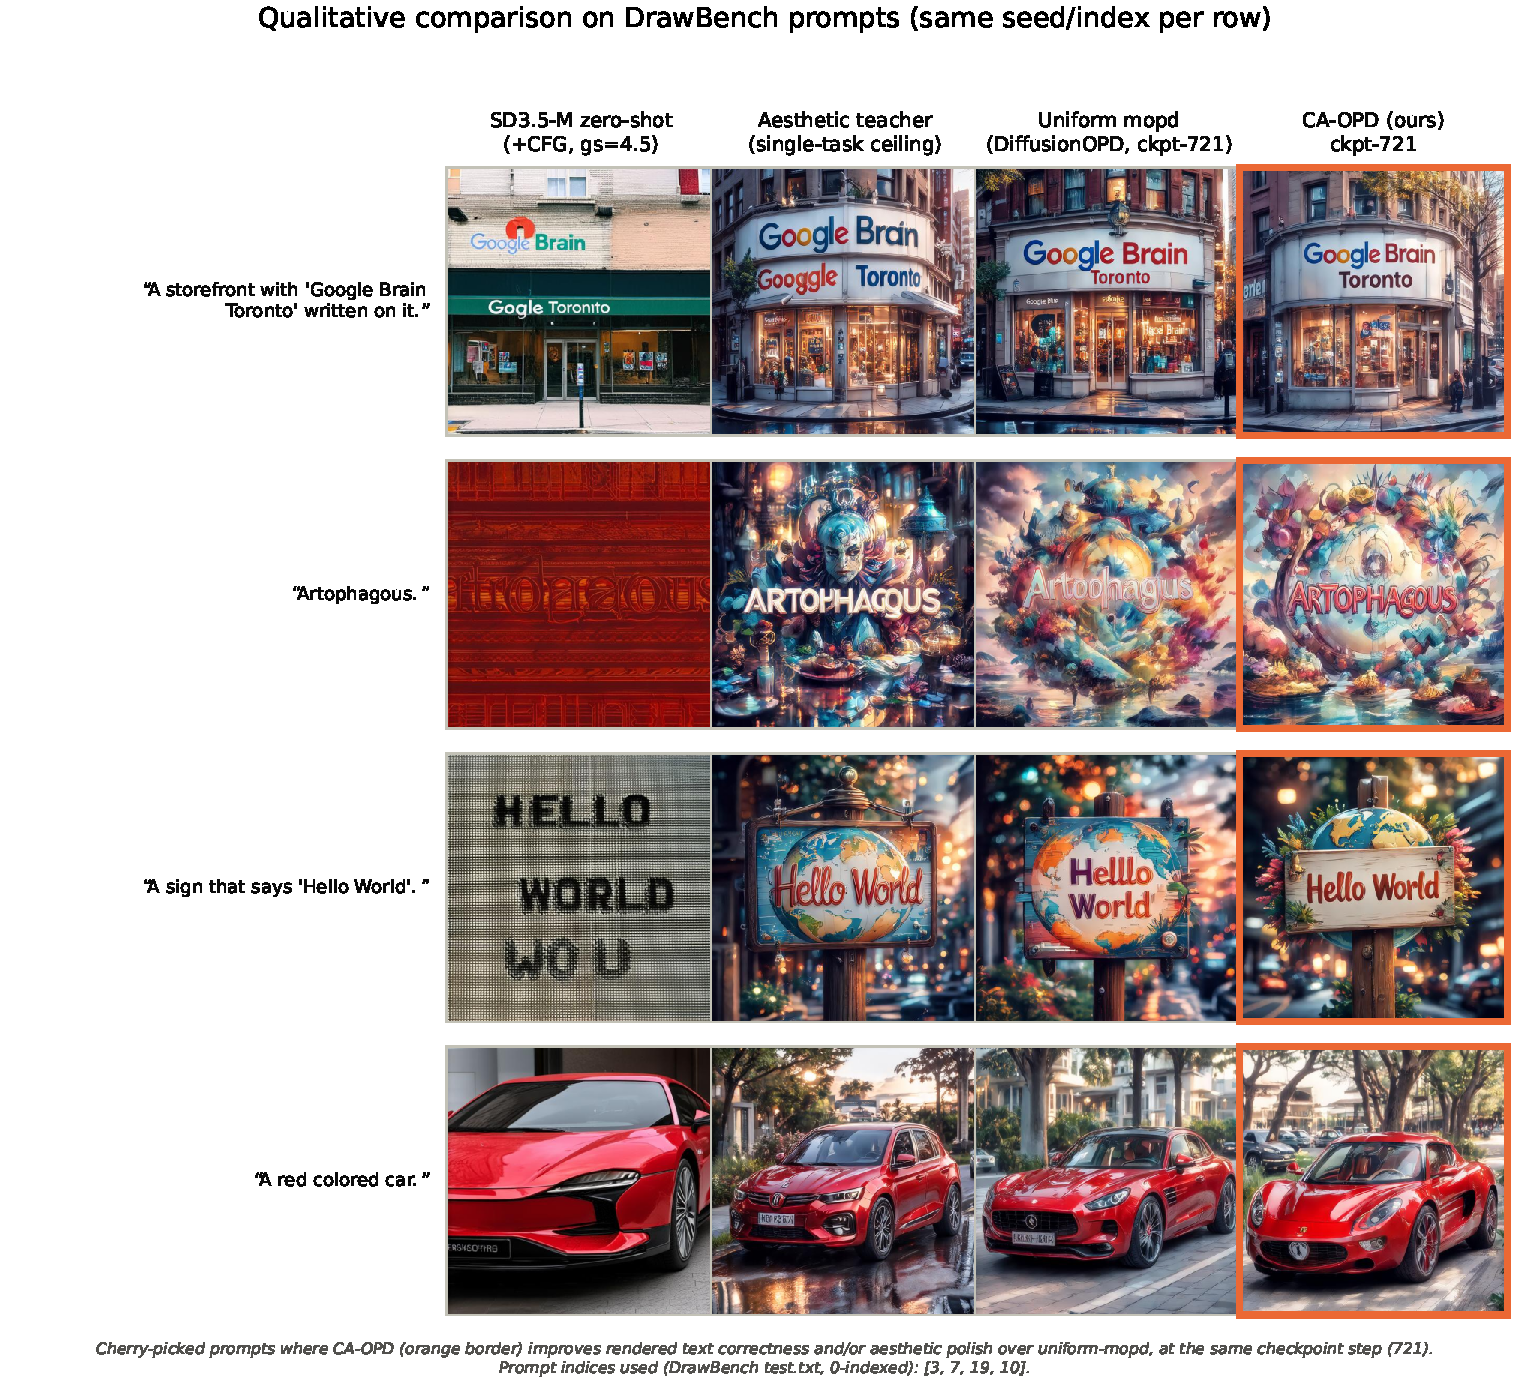
\includegraphics[width=\linewidth]{figures/qualitative.pdf}
  \caption{\textbf{Qualitative comparison} (cherry-picked, shared prompts):
  uniform DiffusionOPD vs.\ CA-OPD at matched steps. CA-OPD reaches a more
  polished aesthetic earlier; convergence-step differences are subtle.}
  \label{fig:qual}
\end{figure}
